\section{Background and Introduction}
\label{sec:intro}  

\section*{Introduction: A reconfigurable reinforcement learning method}

\subsection{RLN MDP structure}
\label{sec:rlnmdpstructure}

The general approach that is taken to form an RLN is ``split'' one single MDP into parent and child processes. Doing so assumes the two process are partly independent [CMDP]. 

\begin{enumerate}[label=\arabic*.]
\item Largely, the models may be independent.
\item The child and parent may include elements of each other's MDP definition in their own definition.
\end{enumerate}

This section focuses on framing a model. In Sections~\ref{sec:mapping} and later, subjects related to behavior optimality, convergence, and computational complexity are considered.

In order to consider the formation of a reconfigurable reinforcement network, it is required to analytically group all aspects of a process and a behavior policy into one tuples.

\begin{center}
\scalebox{0.5}{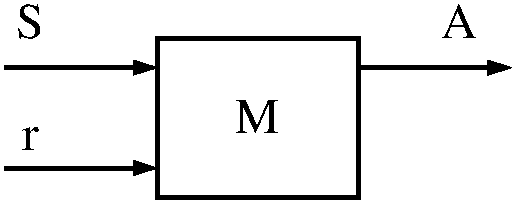
\includegraphics{media/page4diagram.pdf}}
\end{center}

To do this, assume a Markov decision process M which can be internally modeled as a tuple \( M = \langle S, A, T, R, \pi, \tilde{T}, \tilde{R}\rangle \)\\

$S$ -- a set of states $s\in S$ which may be experienced by $M$\\
$A$ -- a set of actions $a\in A$ that may be executed\\
$T$ -- a true transitional probability, $T(s^{\prime}|a,s)$ expressing the probability of executing an action $a$ in state $s$ before ending up in later state $s^{\prime}$.\\
$R$ -- is a reward function which quantifies how desirable a transition $R(s'|a,s)$ is. $R: S\times A \times S\rightarrow \mathbb{R}_{\geq 0}$\\
$\tilde{T}$ -- is the current model of $T$. The goal of $\tilde{T}$ is thus $\tilde{T}\sim T$\\
$\tilde{R}$ -- is the predicted reward of the system, constructed from observation of $R$, s.t.\ $\tilde{R}\rightarrow R$. \\
$\pi$ -- is an action selection policy, ideally chosen to maximize expected reward, an optimal policy is denoted $\pi^*$. Ideally
\begin{equation*}
\pi^*(s) = \argmax_{a}\sum_{s^\prime}\underbrace{R(s^\prime|a,s) T(s'|a,s)+\gamma V(s^\prime)}_{\text{expected reward}}
\end{equation*}
and
\begin{equation*}
\tilde{\pi}(s)  = \argmax_{a}\sum_{s^\prime}\tilde{R}(s^\prime|a,s) \tilde{T}(s'|a,s)+\gamma \tilde{V}(s^\prime)
\end{equation*}

\textbf{[Note that $\tilde{V}$ hasn't been defined in the previous equation.]}

\section*{encoding}

\begin{equation*}
\pi^*(s) = \argmax_{a}\sum_{s^\prime} R(s^\prime|s,a) T(s'|s,a)+\gamma V(s^\prime)
\end{equation*}
where
\begin{equation*}
V(s) = \sum_{s^\prime} R(s^\prime|s,a) T(s^\prime|s,a) +V(s^\prime)\,.
\end{equation*}
A bellman backup can be used [Bellman backup]. In online applications stochastic gradient descent can be applied to regress to locally optimal solutions. This allows estimation of optimal policy
\begin{equation*}
\pi^*(s) = \argmax_{a} Q(s,a)\,.
\end{equation*}

To encode the expected reward over all states, typically $Q$-values are kept: $ Q(s,a) \sim \sum R(s^\prime|a,s)T(s^\prime|a,s)+\gamma V(s^\prime) $ and $ Q_{t+1}(s,a) \leftarrow Q_t(s,a)+\alpha \left( R(s^\prime|a,s)-Q_t(s,a)+\gamma\argmax_{a^\prime} Q(s^\prime,a^\prime) \right) $.

To render the process $M$ separable, it is necessary to decouple the transitional values $T$ from the reward values $R$. Thus, to directly encode $Q(s,a)$ using $\pi$ is prohibitive.\\
knowing: 
\begin{equation*}
Q: S \times A \to \mathbb{R}_{\geq 0}
\end{equation*}
indirect encoding:
\begin{equation*}
\pi: \left\{ S \times A \times S \times \mathbb{N} \middle| R \right\} \to Q
\end{equation*}
If the definitions of $S$ or $A$ change, then $Q$ must be reinitialized. Alternatively, $\tilde{T}$ and $\tilde{R}$ are defined as intermediate encoding functions. Thus we define
\begin{equation*}
\pi:\left\{S \times A \times S \times \mathbb{N}\right\} \to \tilde{T}, \tilde{R}, Q
\end{equation*} 
simple transition
\begin{equation*}
\tilde{T}_{t+1}(s^\prime|s,a) = \frac{\textrm{freq}(s^\prime|s,a)}{\textrm{freq}(s,a)}
\end{equation*}
simple reward
\begin{equation*}
\tilde{R}_{t+1}(s^\prime|s,a) = \tilde{R}(s^\prime|s,a)+\alpha_R\left( \tilde{R}(s^\prime|s,a)-R(s^\prime|s,a)\right)
\end{equation*}
\begin{equation*}
f_Q: \tilde{T}_t \times \tilde{R}_t \to Q_t
\end{equation*}
In this paper we rely on a method of extracting dynamic $Q$-values from an encoded transition and reward function $( \tilde{T}, \tilde{R} )$. The motivation for this encoding is that it allows mapping the transition function into multiple spaces, and allows the reward function to be altered. The significance of this finding is covered in \textbf{???} Price wash \textbf{???}.

 
